%---------- Inleiding ---------------------------------------------------------

\section{Introductie}%
\label{sec:introductie}

Waarover zal je bachelorproef gaan? Introduceer het thema en zorg dat volgende zaken zeker duidelijk aanwezig zijn:

\begin{itemize}
  \item kaderen thema
  \item de doelgroep
  \item de probleemstelling en (centrale) onderzoeksvraag
  \item de onderzoeksdoelstelling
\end{itemize}

Denk er aan: een typische bachelorproef is \textit{toegepast onderzoek}, wat betekent dat je start vanuit een concrete probleemsituatie in bedrijfscontext, een \textbf{casus}. Het is belangrijk om je onderwerp goed af te bakenen: je gaat voor die \textit{ene specifieke probleemsituatie} op zoek naar een goede oplossing, op basis van de huidige kennis in het vakgebied.

De doelgroep moet ook concreet en duidelijk zijn, dus geen algemene of vaag gedefinieerde groepen zoals \emph{bedrijven}, \emph{developers}, \emph{Vlamingen}, enz. Je richt je in elk geval op it-professionals, een bachelorproef is geen populariserende tekst. Eén specifiek bedrijf (die te maken hebben met een concrete probleemsituatie) is dus beter dan \emph{bedrijven} in het algemeen.

Formuleer duidelijk de onderzoeksvraag! De begeleiders lezen nog steeds te veel voorstellen waarin we geen onderzoeksvraag terugvinden.

Schrijf ook iets over de doelstelling. Wat zie je als het concrete eindresultaat van je onderzoek, naast de uitgeschreven scriptie? Is het een proof-of-concept, een rapport met aanbevelingen, \ldots Met welk eindresultaat kan je je bachelorproef als een succes beschouwen?

%---------- Stand van zaken ---------------------------------------------------

\section{State-of-the-art}%
\label{sec:state-of-the-art}

Hier beschrijf je de \emph{state-of-the-art} rondom je gekozen onderzoeksdomein, d.w.z.\ een inleidende, doorlopende tekst over het onderzoeksdomein van je bachelorproef. Je steunt daarbij heel sterk op de professionele \emph{vakliteratuur}, en niet zozeer op populariserende teksten voor een breed publiek. Wat is de huidige stand van zaken in dit domein, en wat zijn nog eventuele open vragen (die misschien de aanleiding waren tot je onderzoeksvraag!)?

Je mag de titel van deze sectie ook aanpassen (literatuurstudie, stand van zaken, enz.). Zijn er al gelijkaardige onderzoeken gevoerd? Wat concluderen ze? Wat is het verschil met jouw onderzoek?

Verwijs bij elke introductie van een term of bewering over het domein naar de vakliteratuur, bijvoorbeeld~\autocite{Hykes2013}! Denk zeker goed na welke werken je refereert en waarom.

Draag zorg voor correcte literatuurverwijzingen! Een bronvermelding hoort thuis \emph{binnen} de zin waar je je op die bron baseert, dus niet er buiten! Maak meteen een verwijzing als je gebruik maakt van een bron. Doe dit dus \emph{niet} aan het einde van een lange paragraaf. Baseer nooit teveel aansluitende tekst op eenzelfde bron.

Als je informatie over bronnen verzamelt in JabRef, zorg er dan voor dat alle nodige info aanwezig is om de bron terug te vinden (zoals uitvoerig besproken in de lessen Research Methods).

% Voor literatuurverwijzingen zijn er twee belangrijke commando's:
% \autocite{KEY} => (Auteur, jaartal) Gebruik dit als de naam van de auteur
%   geen onderdeel is van de zin.
% \textcite{KEY} => Auteur (jaartal)  Gebruik dit als de auteursnaam wel een
%   functie heeft in de zin (bv. ``Uit onderzoek door Doll & Hill (1954) bleek
%   ...'')

Je mag deze sectie nog verder onderverdelen in subsecties als dit de structuur van de tekst kan verduidelijken.

%---------- Methodologie ------------------------------------------------------
\section{Methodologie}%
\label{sec:methodologie}

Voor het onderzoek naar hoe ML/AI kan gebruikt worden om de kwaliteit van artikel master data te verhogen, is een plan van aanpak opgesteld. Dit plan van aanpak is opgesteld in verschillende fases. 

In de eerste fase is het doel om een diepgaande kennis te verwerven over het onderwerp. In de eerste deelfase zal er opzoek gegaan worden naar relevante onderzoek artikelen, academische paper en boeken over hoe de kwaliteit van master data verhoogd kan worden. Daarna zullen de technieken en soort gelijke oplossingen die in eerdere onderzoeken zijn vernomen onderzocht worden. 

Na de eerste fase zullen er duidelijke doelstellingen bepaald worden voor het verder verloop van het onderzoek. In deze fase zullen de verschillende technieken en mogelijkse oplossingen worden vergeleken met elkaar en zal er nagegaan worden of deze oplossingen rendabel genoeg zijn om zelf op de markt te brengen en zelf te ontwerpen. Ook zal er onderzoek verricht worden naar de specifieke concurrentie van deze mogelijkse oplossingen. 

Na deze fase zal de techniek of oplossing gekozen worden. Deze techniek of oplossing zal geselecteerd worden aan de hand van de doelstellingen die in voorgaande fases zijn vastgelegd. Als eerste zal er onderzoek gedaan worden naar welk neutraal netwerk er nodig zal zijn. Als tweede zal er gezocht moeten naar al dan niet bestaande libraries die we kunnen gebruiken en welke de beste is.

In de volgende fase zal er een dataset verzameld worden. Het verzamelen van een representatieve dataset is essentieel voor het succes van het onderzoek. Er zal opzoek moeten gegaan worden naar een dataset met een brede scala aan master data zodat de kwaliteit van onze oplossing kan getest worden. Om een goede dataset te vinden zal deze samengesteld worden aan de hand van datasets van specifieke bedrijven die veel gebruik maken van material master data.

In de vijfde fase zal er een proof-of-concept uitgewerkt worden. Gebaseerd op het onderzoek zal er een proof-of-concept ontworpen worden, die de kwaliteit van master data mogelijks kan verhogen. De nodige middelen zullen afhankelijk zijn van welke oplossing er uit het onderzoek is gekomen. De oplossing zal getraind worden aan de hand van de verzamelde dataset. 

Na de uitwerking van de proof-of-concept zal er onderzoek verricht worden naar hoe deze oplossing makkelijk in de SAP master data governance (MDG) tool kan geïntegreerd worden. Er zal gekeken worden naar waar en hoe we dit best implementeren om de uitwerking ervan optimaal te kunnen benutten.

Als laatste zal er een conclusie worden getrokken uit het onderzoek en een antwoord worden geformuleerd op de onderzoeksvraag op basis van de verkregen resultaten. Ook zal er een aanbeveling worden geschreven voor de implementatie van de meest efficiënte en rendabelste techniek om de kwaliteit van artikel master data te verhogen. 

\begin{center}
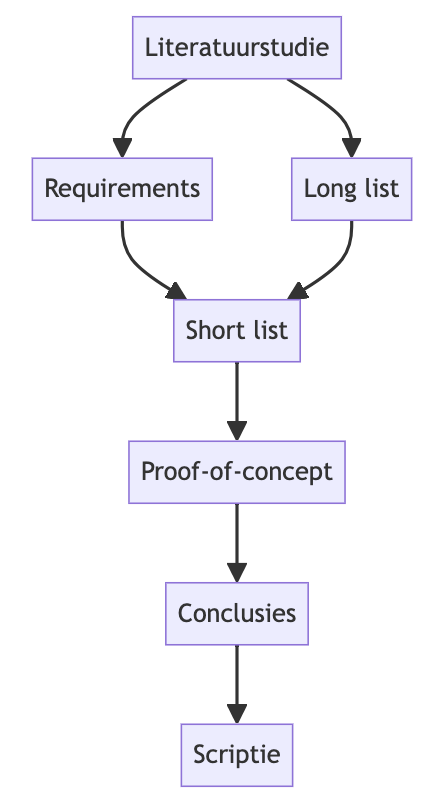
\includegraphics[scale=0.5]{methodologie.png}
\end{center}

%---------- Verwachte resultaten ----------------------------------------------
\section{Verwacht resultaat, conclusie}%
\label{sec:verwachte_resultaten}

Hier beschrijf je welke resultaten je verwacht. Als je metingen en simulaties uitvoert, kan je hier al mock-ups maken van de grafieken samen met de verwachte conclusies. Benoem zeker al je assen en de onderdelen van de grafiek die je gaat gebruiken. Dit zorgt ervoor dat je concreet weet welk soort data je moet verzamelen en hoe je die moet meten.

Wat heeft de doelgroep van je onderzoek aan het resultaat? Op welke manier zorgt jouw bachelorproef voor een meerwaarde?

Hier beschrijf je wat je verwacht uit je onderzoek, met de motivatie waarom. Het is \textbf{niet} erg indien uit je onderzoek andere resultaten en conclusies vloeien dan dat je hier beschrijft: het is dan juist interessant om te onderzoeken waarom jouw hypothesen niet overeenkomen met de resultaten.

